
\documentclass[letterpaper, 10 pt, conference]{ieeeconf}  
\IEEEoverridecommandlockouts                             
\usepackage{graphicx} 
\usepackage{hyperref}

\overrideIEEEmargins

\title{\Huge Dense Optic Flow}
\author{Jiyu Tian} 

\begin{document}

\maketitle
\thispagestyle{empty}
\pagestyle{empty}

%-------------------------------------------------------------------------

\section{INTRODUCTION}
In this project we explore the implementation of the Lucas-Kanade method for estimating dense optic flow from a pair of images. We take a pair of greyscale images taken from a video sequence as the input, and output two matrices containing the x and y components of the flow vector at each pixel.
%-------------------------------------------------------------------------
\section{ALGORITHMS DESCRIPTION}
\subsection{Grayscale Conversion}
After reading in two images, we first make them grayscale.We apply the conversion as the following eqaution:
\begin{equation}
Gray = 0.299 \times R + 0.587 \times G + 0.114 \times B
\end{equation}

If, in the worst case, input images do not have all the three $RGB$ channels, we simply regard the first channel as its grayscale value.
\subsection{Image Gradient}
Before taking the derivative, we smooth the images using Gaussian filter. The spatial intensity gradients $I_x$ and $I_y$ of second image is computed using horizontal and vertical components of Prewitt/Sobel mask. Compute the temporal gradient $I_t$ by subtracting a smoothed version of first image from a smoothed version of the second image.
\subsection{Lucas-Kanade Method}
For a given $N\times N$ window, a system of linear equations can be formed at each pixel by summing over products of gradients in its neighborhood. That is, at each pixel, we have a set of equations:
\begin{equation}
\left[ \begin{array}{cc}
\sum I^2_x & \sum I_xI_y\\
\sum I_xI_y & \sum I^2_y
\end{array} \right] \left[ \begin{array}{c}
V_x\\
V_y
\end{array} \right]= -\left[ \begin{array}{c}
\sum I_xI_t\\
\sum I_yI_t
\end{array} \right]
\end{equation}

The flow vector $[V_x, \ V_y]$ can then be solved at each pixel.
%-------------------------------------------------------------------------
\section{EXPERIMENTAL RESULTS}



%-------------------------------------------------------------------------
\section{CONCLUSION}
In this project, we explored various application of feature matching, and creatively applied them to image mosaicing. This is a very useful technique for constructing panoramic image mosaics from sequences of images.
\vfill

\end{document}


\begin{figure}[thpb]
\centering
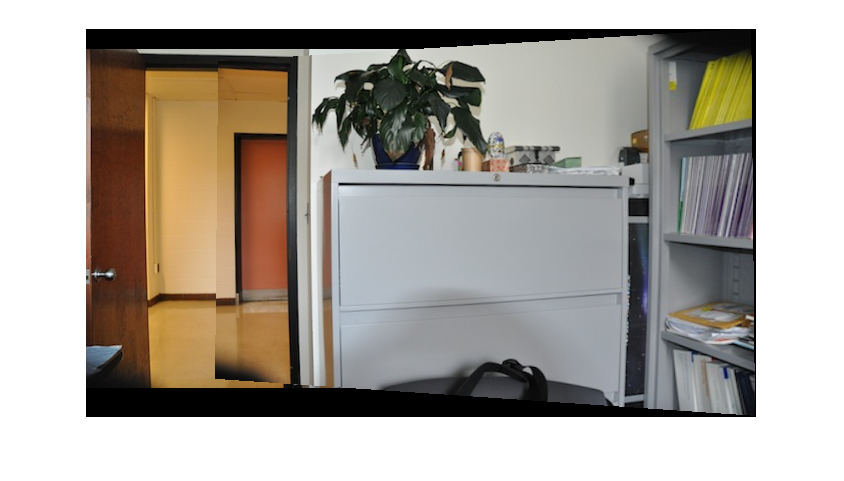
\includegraphics[width=0.4\textwidth]{mosaic.png}
\caption{Final Mosaic}
\label{mosaic}
\end{figure}


